\documentclass[10pt]{article}
\usepackage[a4paper]{geometry}
\usepackage[footnotesize]{caption}
\usepackage{longtable}
\usepackage{booktabs}
\usepackage{hyperref}
\usepackage{enumitem}
\usepackage{marginnote}
\usepackage{listings}
\usepackage[tikz,math]{forsyde}

\title{The \ForSyDeLaTeX utilities}
\author{
  George Ungureanu \\
  Department of Electronic Systems\\
  KTH Royal Institute of Technology\\
  Stockholm, SWEDEN
}
\date{\today}



\newenvironment{optionslist}[0]{ 
\begin{list}{}{
	\setlength{\itemindent}{-10pt}
%	\setlength{\topsep}{0pt}
	\setlength{\itemsep}{0pt}
	\setlength{\parsep}{0pt}
}}{\end{list}}
\newcommand\bookmark[1]{\marginpar{\ttfamily #1}}
\lstset{
  basicstyle=\footnotesize\ttfamily,
  % numbers=left,
  frame=single,
  numberstyle=\tiny\color{black!30},
  commentstyle=\color{blue}\textit,
  stringstyle=\color{magenta}\textit,
  flexiblecolumns=false,
  basewidth={0.5em,0.45em},
  breaklines=true,
  language={[LaTeX]TeX},
  texcsstyle=*\color{red}\bfseries,
  keywordstyle=\color{blue}\bfseries,
  morekeywords={tikzpicture,document},
  moretexcs={trans,standard,interface,basic,cluster,node,path,embed},
}
\def\opt#1{\color{gray}{#1}}
\def\man#1{\color{black}{#1}}

\begin{document}
\maketitle
\reversemarginpar

\begin{abstract}
This is the reference manual for the \LaTeX\ utilities used in the context of \ForSyDe. All packages and their API features are documented here.
\end{abstract}

\section{Introduction}

This library was developed as an effort to standardize symbols and graphical primitives in documents related to \textsc{ForSyDe}, but also to provide tools and utilities for user convenience. \ForSyDe is a high-level design methodology aiming at synthesizing correct-by-construction systems through formal means. For more information check \url{https://forsyde.ict.kth.se}.

The library contains the following main packages:
\begin{itemize}
\item \texttt{forsyde-tikz} : is a collection of \textsc{PGF} and \textsc{TikZ} styles, graphical primitives and commands for drawing \textsc{ForSyDe} process networks;
\item \texttt{forsyde-math} : is a collection of math symbols used in the \textsc{ForSyDe} formal notation. It is mainly focused on the ongoing \textsc{ForSyDe-Atom} methodology;
\item \texttt{forsyde-plot} : provides utilities for plotting \textsc{ForSyDe} signals;
\item \texttt{forsyde-legacy} : API for the previous versions of this library.
\end{itemize}

\section{Installation \& usage}

There are three main alternatives to install the libraries:

\begin{enumerate}
\item copy the contents of \texttt{forsyde-latex/src} in its appropriate path under the \texttt{TEXMFHOME} path or any standard loading path, as specified by your \LaTeX\ compiler. Refer to \url{https://en.wikibooks.org/wiki/LaTeX/Installing_Extra_Packages} for more information.
\item compile your document with the variable \texttt{TEXINPUTS} set to \texttt{/path/to/forsyde-latex/src/}; % and \texttt{TEXFONTS} set to \texttt{/path/to/forsyde-latex/fonts/}
\item copy the contents of \texttt{forsyde-latex/src} in the same folder as your document and compile normally.
\end{enumerate}

To include any of the packages enumerated in the introduction, you cal load the \texttt{forsyde} package with the appropriate option:

\begin{verbatim}
	\usepackage[option]{forsyde}
\end{verbatim}
where \texttt{option} is
\begin{itemize}
\item \texttt{tikz} for loading the \texttt{forsyde-tikz} library
\item \texttt{math} for loading the \texttt{forsyde-math} library
\item \texttt{plot} for loading the \texttt{forsyde-plot} library
\item \texttt{legacy} for loading the \texttt{forsyde-legacy} library
\end{itemize}

When loaded without an option, this package only provides some general commands for typesetting and logos (TBA):

\begin{longtable} { c | c }
  \toprule
  \textbf{Command}  & \textbf{Expands to} \\
  \midrule
  \texttt{\string\ForSyDe}      & \ForSyDe \\
  \texttt{\string\ForSyDeLaTeX} & \ForSyDeLaTeX \\
  \bottomrule
\end{longtable}

\newpage
\tableofcontents
\newpage
% A library with graphical primitives for ForSyDe process networks
%
% Author: George Ungureanu, KTH - Royal Institute of Technology, Sweden
% Version: 0.3
% Date: 2015/05/20
\NeedsTeXFormat{LaTeX2e}
\RequirePackage{pgfplots}
\RequirePackage{pgfkeys}
\RequirePackage{xparse,l3regex}
\RequirePackage{ezkeys}
\RequirePackage{xstring}
\usetikzlibrary{decorations.markings, shapes, positioning, calc, fit, backgrounds, intersections, arrows}

\ProvidesPackage{forsyde-tikz}
              [2015/05/20 v0.3 ForSyDe TikZ Library]

\usetikzlibrary{fkeys,fshapes,fpaths,fnodes}


%%%%%%%%%%%%%
% CONSTANTS %
%%%%%%%%%%%%%
% Colors
\newcommand{\defaultdrawcolor}{black}     		% draw color of signal paths
\newcommand{\defaultfillcolor}{white}     		% draw color of signal paths
\definecolor{sycolor}{RGB}{148,183,215}
\definecolor{ctcolor}{RGB}{225,119,19}
\definecolor{decolor}{RGB}{80,229,154}
\definecolor{sdfcolor}{RGB}{220,220,20}
\definecolor{blackboxcolor}{gray}{0.80}
% line widths of
\newlength{\sepq}\pgfmathsetlength{\sepq}{2pt}
\newcommand{\compositelinewidth}{.4pt}       % composite process line width
\newcommand{\skeletonlinewidth}{1pt}         % parallel processes line width
\newcommand{\signalpathlinewidth}{1pt}       % signal paths
\newcommand{\functionpathlinewidth}{.8pt}    % function paths
\newcommand{\vectorpathlinewidth}{3pt}       % vector paths
% sizes, etc.
\newcommand{\tokensize}{2pt}
\newcommand{\halftokensize}{1pt}

%%%%%%%%%%%%%%%%%%%%%%%%
% GENERIC TIKZ HELPERS %
%%%%%%%%%%%%%%%%%%%%%%%%
% Positioning of node text.
% #1 = node label
% #2 = label text
\newcommand{\textaboveof}[2]{\pgftext[bottom,at=\pgfpointanchor{#1}{north},y=+1mm]{#2}}%
\newcommand{\textrightof}[2]{\pgftext[left,  at=\pgfpointanchor{#1}{east}, x=+1mm]{#2}}%
\newcommand{\textbelowof}[2]{\pgftext[top,   at=\pgfpointanchor{#1}{south},y=-1mm]{#2}}%
\newcommand{\textleftof} [2]{\pgftext[right, at=\pgfpointanchor{#1}{west}, x=-1mm]{#2}}%


% Conditional if node was defined.
% #1 = node label
% #2 = true-statement
% #3 = false-statement
\long\def\ifnodedefined#1#2#3{%
    \@ifundefined{pgf@sh@ns@#1}{#3}{#2}%
}

\newcommand{\gettikzx}[2]{%
  \tikz@scan@one@point\pgfutil@firstofone#1\relax
  \edef#2{\the\pgf@x}%
}
% Get y-coordinate of node
\newcommand{\gettikzy}[2]{%
  \tikz@scan@one@point\pgfutil@firstofone#1\relax
  \edef#2{\the\pgf@y}%
}
% Get x- and y- coordinate of node
\newcommand{\gettikzxy}[3]{%
  \tikz@scan@one@point\pgfutil@firstofone#1\relax
  \edef#2{\the\pgf@x}%
  \edef#3{\the\pgf@y}%
}

% Decorate process ports with info
% #1 = node label
\newcounter{iportnum}
\newcounter{oportnum}
\newcommand\resetportinfo[1]{%
  \setcounter{iportnum}{0}
  \setcounter{oportnum}{0}
  \def\currentnode{#1}
}
\newcommand\wpinfo[2][south east]{%
  \addtocounter{iportnum}{1}
  \node[anchor=#1] at (\currentnode.w\theiportnum) {\tiny #2};
}
\newcommand\epinfo[2][south west]{%
  \addtocounter{oportnum}{1}
  \node[anchor=#1] at (\currentnode.e\theoportnum) {\tiny #2};
}


\tikzset{% 
    anch/.style={circle, draw=none, fill=red, inner sep=0pt, minimum size=3pt},
    label/.style={font=\ttfamily\scriptsize, text=red}
}




%%%%%%%%%%%%%%%%%%%%%%%%%%% 
% SHAPES OF MAIN ELEMENTS %
%%%%%%%%%%%%%%%%%%%%%%%%%%% 
\pgfkeys{/forsyde keys/.is family, /forsyde keys,
  primitive/.style ={%
    shape=atom shape
    },
  primitiven/.style={%
    shape=nary atom shape
    },
  leaf/.style={%
    hasmoc,
    shape=leaf shape,
    },
  leafn/.style={% 
    hasmoc,
    shape=leafn shape,
    },
  composite/.style={%
    shape=comp shape
    },
  compositen/.style={%
    shape=nary comp shape,
    },
  embed/.style={%
    hasmoc,
    shape=leaf shape,
    inner sep=15pt,
    },
  farmstyle/.style={%
    shape = dp shape,
    inner xsep = 15pt,
    inner ysep = 20pt,
    },
  pipestyle/.style={%
    shape = pipe shape,
    inner xsep = 15pt,
    inner ysep = 20pt,
    },
  skeleton/.style={%
    shape = generic skel shape,
    inner xsep = 15pt,
    inner ysep = 20pt,
    },
  transition/.code 2 args = {%
    \edef\theshape{trans shape #1#2}
    \tikzset{/forsyde keys/shape = \theshape}
    },
  transition/.default={v1}{v1},
  zipx/.style = {%
    transition={s1}{v1},
    rotate shape=180,
    type=zipx,
    },
  unzipx/.style = {%
    transition={s1}{v1},
    type=unzipx,
    },    
}
\newpage
\vfill
\begin{figure}[htb]\centering
  {%
    \setlength{\fboxsep}{7pt}%
    \setlength{\fboxrule}{1pt}%
    \fbox{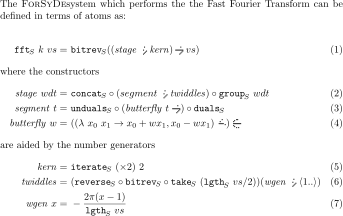
\includegraphics[width=.9\textwidth]{figs/example-forsyde-math}}
  }
\end{figure}
\lstinputlisting{figs/example-forsyde-math.tex}
\vfill
\newpage

\section{The \texttt{forsyde-math} package}
\label{sec:forsyde-math-package}

This package provides a set of symbols and commands for writing equations mainly for the \ForSyDeAtom\ theoretical framework.

\subsection{Symbol Fonts}
\label{sec:fonts}

All \ForSyDeAtom\ operators have been bundled in a font family called \texttt{forsydeatom}, which can be used imported in accordance to the \LaTeXe\ standard. The math symbol font is called \texttt{atomoperators} and it is based on the \texttt{forsydeatom} font family.

The \texttt{forsyde-math} imports these fonts and provides macros for typing them in math or texst environments.

\def\makesymbolrow#1{{\tiny #1} & {\scriptsize #1} & {\footnotesize #1} & {\small #1} & {\normalsize #1} & {\large #1} & {\Large #1} & {\LARGE #1} & {\huge #1} & {\Huge #1}}
\begin{longtable} { c | c c c c c c c c c c }
  \toprule
  \textbf{Command}  & \textbf{5pt} & \textbf{7pt} & \textbf{8pt} & \textbf{9pt} & \textbf{10pt} & \textbf{12pt} & \textbf{14.4pt} & \textbf{17.28pt} & \textbf{20.74pt} & \textbf{24.88pt} \\
  \midrule
  \texttt{\string\BhFun} & \makesymbolrow{\textBhFun} \\
  \texttt{\string\BhApp} & \makesymbolrow{\textBhApp} \\
  \texttt{\string\BhDef} & \makesymbolrow{\textBhDef} \\
  \texttt{\string\BhPhi} & \makesymbolrow{\textBhPhi} \\
  \midrule
  \texttt{\string\MocFun} & \makesymbolrow{\textMocFun} \\
  \texttt{\string\MocApp} & \makesymbolrow{\textMocApp} \\
  \texttt{\string\MocCmb} & \makesymbolrow{\textMocCmb} \\
  \texttt{\string\MocPre} & \makesymbolrow{\textMocPre} \\
  \texttt{\string\MocPhi} & \makesymbolrow{\textMocPhi} \\
  \texttt{\string\MocDel} & \makesymbolrow{\textMocDel} \\
  \midrule
  \texttt{\string\SkelFrm} & \makesymbolrow{\textSkelFrm} \\
  \texttt{\string\SkelPip} & \makesymbolrow{\textSkelPip} \\
  \texttt{\string\SkelFun} & \makesymbolrow{\textSkelFun} \\
  \texttt{\string\SkelApp} & \makesymbolrow{\textSkelApp} \\
  \texttt{\string\SkelRed} & \makesymbolrow{\textSkelRed} \\
  \texttt{\string\SkelRec} & \makesymbolrow{\textSkelRec} \\
  \bottomrule
\end{longtable}


%%% Local Variables:
%%% TeX-command-default: "Make"
%%% mode: latex
%%% TeX-master: "../refman"
%%% End:

\newpage
\section{The \texttt{forsyde-legacy} package}
\label{sec:legacy-package}

This package offers an API for the legacy commands defined in older versions of the \ForSyDeLaTeX utilities. This way, documents compiled with old commands can be compiled with the newer versions of their respective library.

\subsection{\texttt{forsyde-tikz v0.3} or prior}
\label{sec:forsyde-tikz-v0.3}

Although from \texttt{v0.4} onward the draw commands have been heavily modified, the old commands could be mapped to the new API.

\begin{lstlisting}
\primitive[keys]         {id}{pos}{label}
\primitiven[keys]        {id}{pos}{label}
\leafstd[keys]           {id}{pos}{label}
\leafcustom[keys]        {id}{pos}
\compositestd[keys]      {id}{clustered nodes}{label}
\compositebbox[keys]     {id}{pos}{label}
\patterncluster[keys]    {id}{clustered nodes}{label}
\patternnodestd[keys]    {id}{pos}
\patternnodecustom[keys] {id}{pos}
\end{lstlisting}

\subsection{\texttt{forsyde-pc v0.3} or prior}
\label{sec:forsyde-pc-v0.3}

This package is obsolete and used to hold helpers associated to some \ForSyDe process constructors.

\begin{lstlisting}
\delay    [moc=,f1=,inner sep=,reverse]        {id}{pos}{label}
\delayn   [moc=,f1=,f2=,inner sep=,reverse]    {id}{pos}{label}
\map      [moc=,f1=,inner sep=,reverse]        {id}{pos}{label}
\comb     [moc=,f1=,inner sep=,reverse]        {id}{pos}{label}
\combII   [moc=,f1=,inner sep=,reverse]        {id}{pos}{label}
\combIII  [moc=,f1=,inner sep=,reverse]        {id}{pos}{label}
\combIV   [moc=,f1=,inner sep=,reverse]        {id}{pos}{label}
\scanl    [moc=,f1=,f2=,inner sep=,reverse]    {id}{pos}{label}
\scanlII  [moc=,f1=,f2=,inner sep=,reverse]    {id}{pos}{label}
\scanlIII [moc=,f1=,f2=,inner sep=,reverse]    {id}{pos}{label}
\scanld   [moc=,f1=,f2=,f3=,inner sep=,reverse]{id}{pos}{label}
\scanldII [moc=,f1=,f2=,f3=,inner sep=,reverse]{id}{pos}{label}
\scanldIII[moc=,f1=,f2=,f3=,inner sep=,reverse]{id}{pos}{label}
\moore    [moc=,f1=,f2=,f3=,inner sep=,reverse]{id}{pos}{label}
\mooreII  [moc=,f1=,f2=,f3=,inner sep=,reverse]{id}{pos}{label}
\mooreIII [moc=,f1=,f2=,f3=,inner sep=,reverse]{id}{pos}{label}
\mealy    [moc=,f1=,f2=,f3=,inner sep=,reverse]{id}{pos}{label}
\mealyII  [moc=,f1=,f2=,f3=,inner sep=,reverse]{id}{pos}{label}
\mealyIII [moc=,f1=,f2=,f3=,inner sep=,reverse]{id}{pos}{label}
\source   [moc=,f1=,f2=,inner sep=,reverse]    {id}{pos}{label}
\filter   [moc=,f1=,f2=,inner sep=,reverse]    {id}{pos}{label}
\hold     [moc=,f1=,inner sep=,reverse]        {id}{pos}{label}
\fillS    [moc=,f1=,f2=,inner sep=,reverse]    {id}{pos}{label}

\zip     [moc=,reverse]{id}{pos}
\zipIII  [moc=,reverse]{id}{pos}
\zipIV   [moc=,reverse]{id}{pos}
\zipV    [moc=,reverse]{id}{pos}
\zipVI   [moc=,reverse]{id}{pos}
\unzip   [moc=,reverse]{id}{pos}
\unzipIII[moc=,reverse]{id}{pos}
\unzipIV [moc=,reverse]{id}{pos}
\unzipV  [moc=,reverse]{id}{pos}
\unzipVI [moc=,reverse]{id}{pos}

\domaininterface[moc=,reverse]          {id}{pos}
\mocinterface   [mocin=,mocout=,reverse]{id}{pos}

\composite[ni=,no=,inner xsep=,inner ysep=,reverse] {id}{included}{label}
\blackbox [ni=,no=,inner xsep=,inner ysep=,reverse] {id}{included}{label}

\farm     [ni=,no=,inner xsep=,inner ysep=,reverse]                {id}{included}{label}
\farmI    [ni=,no=,f1=,inner xsep=,inner ysep=,reverse]            {id}{included}{label}
\farmII   [ni=,no=,f1=,f2=,inner xsep=,inner ysep=,reverse]        {id}{included}{label}
\farmIII  [ni=,no=,f1=,f2=,f3=,inner xsep=,inner ysep=,reverse]    {id}{included}{label}
\farmIV   [ni=,no=,f1=,f2=,f3=,f4=,inner xsep=,inner ysep=,reverse]{id}{included}{label}
\pipe     [ni=,no=,inner xsep=,inner ysep=,reverse]                {id}{included}{label}
\pipeI    [ni=,no=,f1=,inner xsep=,inner ysep=,reverse]            {id}{included}{label}
\pipeII   [ni=,no=,f1=,f2=,inner xsep=,inner ysep=,reverse]        {id}{included}{label}
\pipeIII  [ni=,no=,f1=,f2=,f3=,inner xsep=,inner ysep=,reverse]    {id}{included}{label}
\pipeIV   [ni=,no=,f1=,f2=,f3=,f4=,inner xsep=,inner ysep=,reverse]{id}{included}{label}
\reduce   [ni=,no=,inner xsep=,inner ysep=,reverse]                {id}{included}{label}
\reduceI  [ni=,no=,f1=,inner xsep=,inner ysep=,reverse]            {id}{included}{label}
\reduceII [ni=,no=,f1=,f2=,inner xsep=,inner ysep=,reverse]        {id}{included}{label}
\reduceIII[ni=,no=,f1=,f2=,f3=,inner xsep=,inner ysep=,reverse]    {id}{included}{label}
\reduceIV [ni=,no=,f1=,f2=,f3=,f4=,inner xsep=,inner ysep=,reverse]{id}{included}{label}

\unzipx     [reverse]         {id}{position}
\zipx       [reverse]         {id}{position}
\unzipv     [reverse]         {id}{position}
\zipv       [reverse]         {id}{position}
\splitatv   [f1=,reverse]     {id}{position}
\catv       [reverse]         {id}{position}
\oddsv      [reverse]         {id}{position}
\evensv     [reverse]         {id}{position}
\reversev   [reverse]         {id}{position}
\groupv     [reverse]         {id}{position}
\concatv    [reverse]         {id}{position}
\filteridxv [f1=,reverse]     {id}{position}
\gatherv    [f1=,f2=,reverse] {id}{position}
\gatherAdpv [f1=,f2=,reverse] {id}{position}
\selectv    [reverse]         {id}{position}
\distributev[f1=,reverse]     {id}{position}
\filterv    [f1=,reverse]     {id}{position}
\getv       [f1=,reverse]     {id}{position}

\visualoddsv   [reverse]{id}{pos}
\visualevensv  [reverse]{id}{pos}
\visualreversev[reverse]{id}{pos}
\visualgroupv  [reverse]{id}{pos}
\visualconcatv [reverse]{id}{pos}
\end{lstlisting}


%%% Local Variables:
%%% TeX-command-default: "Make"
%%% mode: latex
%%% TeX-master: "../refman"
%%% End:



\end{document}
%%% Local Variables:
%%% TeX-command-default: "Make"
%%% mode: latex
%%% TeX-master: t
%%% End:
